
\documentclass[11pt]{article}
% ------- TikZ Preamble -------
\RequirePackage{tikz}
\usetikzlibrary{knots,hobby,calc,arrows.meta,intersections,decorations.pathreplacing,decorations.markings,shapes.geometric,spath3}
\usepackage{amsmath}
\usepackage{hyperref}
\usepackage{calc,pict2e}
% stix replaces amssymb/amsfonts; loading both exceeds the symbol-font limit ("Too many symbol fonts declared").
\usepackage{stix}

\newcommand{\SSTGuidesPoints}[2]{% #1=basename (e.g. P), #2=last index
    \ifsstguides
    \foreach \i in {1,...,#2}{
        \fill[blue] (#1\i) circle (1.2pt);
        \node[blue,font=\scriptsize,above] at (#1\i) {\i};
    }
    \draw[gray!40, dashed]
    \foreach \i [remember=\i as \lasti (initially 1)] in {2,...,#2,1} { (#1\lasti)--(#1\i) };
    \fi
}

\tikzset{
    knot diagram/every strand/.append style={
        ultra thick,
        black
    },
    show curve controls/.style={
        postaction=decorate,
        decoration={show path construction,
        curveto code={
            \draw [blue, dashed]
            (\tikzinputsegmentfirst) -- (\tikzinputsegmentsupporta)
            node [at end, draw, solid, red, inner sep=2pt]{};
            \draw [blue, dashed]
            (\tikzinputsegmentsupportb) -- (\tikzinputsegmentlast)
            node [at start, draw, solid, red, inner sep=2pt]{}
            node [at end, fill, blue, ellipse, inner sep=2pt]{}
            ;
        }
        }
    },
    show curve endpoints/.style={
        postaction=decorate,
        decoration={show path construction,
        curveto code={
            \node [fill, blue, ellipse, inner sep=2pt] at (\tikzinputsegmentlast) {}
            ;
        }
        }
    }
}



% Document
\begin{document}
\subsection{Chiral Torus Knots}
    \begin{table}[h!]
      \centering
      \label{tab:trefoil-variants}
      \begin{tabular}{c c}
        \textbf{$T_{(3,2)}$ Left handed}  & \textbf{Right handed $T_{(2,3)}$} \\
        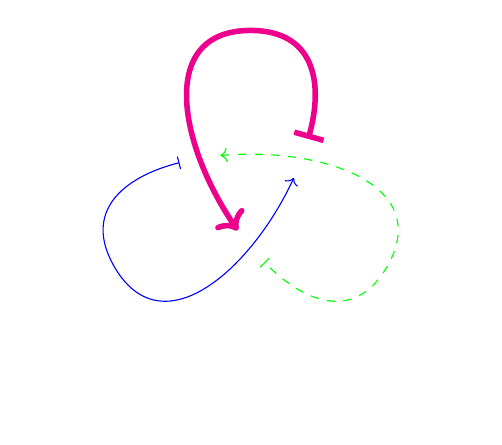
\begin{tikzpicture}
            \path[spath/save=trefoil]
            (0,2) .. controls +(2.2,0) and +(120:-2.2) ..
            (210:2) .. controls +(120:2.2) and +(60:2.2) ..
            (-30:2) .. controls +(60:-2.2) and +(-2.2,0) .. (0,2);
            \tikzset{
                every trefoil component/.style={draw},
                trefoil component 1/.style={blue, <-|},
                trefoil component 2/.style={green, dashed, <-|},
                trefoil component 3/.style={magenta, line width=2pt,  <-|},
                spath/knot={trefoil}{15pt}{1,3,5},
            }
        \end{tikzpicture}
        &
        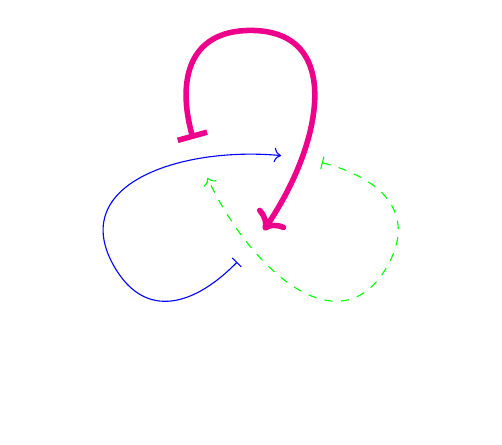
\begin{tikzpicture}
            \path[spath/save=trefoil]
            (0,2) .. controls +(2.2,0) and +(120:-2.2) ..
            (210:2) .. controls +(120:2.2) and +(60:2.2) ..
            (-30:2) .. controls +(60:-2.2) and +(-2.2,0) .. (0,2);
            \tikzset{
              every trefoil component/.style={draw},
              trefoil component 1/.style={blue, |->},
              trefoil component 2/.style={green, dashed, |->},
              trefoil component 3/.style={magenta, line width=2pt, |->},
              spath/knot={trefoil}{15pt}{2,4,6},
            }
        \end{tikzpicture}
      \end{tabular}
    \end{table}

    \subsection{Torus Knots variants}
    \begin{table}[h!]
        \centering
        \label{tab:torusknot-variants-3-5}
        \begin{tabular}{c c c}
          \textbf{$3_1$ Trefoil} & \textbf{$5_1$ Cinquefoil} & \textbf{$7_1$ Septafoil } \\
          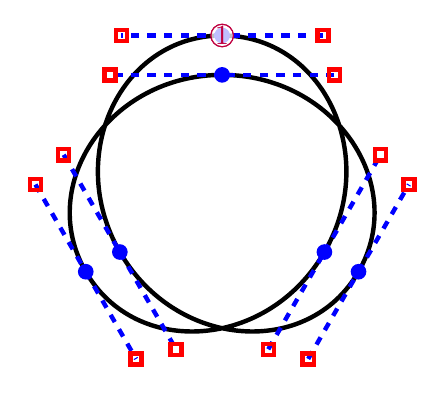
\begin{tikzpicture}[use Hobby shortcut]
                \begin{knot}[
                    consider self intersections=true,
                    draft mode=crossings,
                    flip crossing/.list={2,4},
                    only when rendering/.style={show curve controls}
                ]
                     \strand ([closed]90:2) foreach \k in {1,...,3}  { .. (90-360/3+ \k*720/3: 1.5) .. (90+\k*720/3: 2) } (90:2);
                \end{knot}
          \end{tikzpicture}
          &
          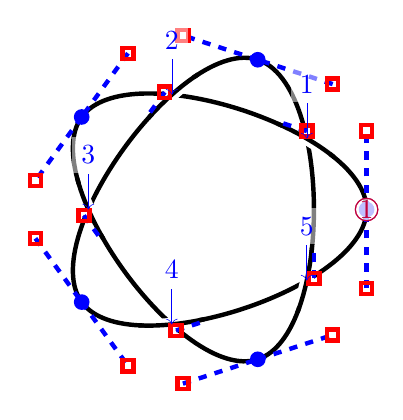
\begin{tikzpicture}
              \begin{knot}[
                  consider self intersections=true,
                  draft mode=crossings,
                  flip crossing/.list={2,4},
                  only when rendering/.style={show curve controls}
              ]
                  \strand (2,0) .. controls +(0,1.0) and +(54:1.0) .. (144:2) .. controls +(54:-1.0) and +(18:-1.0) .. (-72:2) .. controls +(18:1.0) and +(162:-1.0) .. (72:2) .. controls +(162:1.0) and +(126:1.0) .. (-144:2) .. controls +(126:-1.0) and +(0,-1.0) .. (2,0);
              \end{knot}
          \end{tikzpicture}
        &
          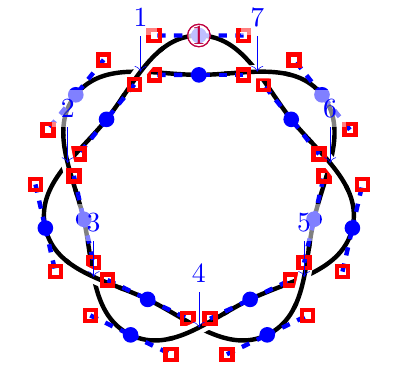
\begin{tikzpicture}[use Hobby shortcut]
                \begin{knot}[
                    consider self intersections=true,
                    draft mode=crossings,
                    flip crossing/.list={2,4,6},
                    only when rendering/.style={show curve controls}
                ]
                    \strand ([closed]90:2) foreach \k in {1,...,7}  { .. (90-360/7+ \k*720/7: 1.5) .. (90+\k*720/7: 2) } (90:2);
                \end{knot}
          \end{tikzpicture}
        \end{tabular}
    \end{table}


    \begin{table}[h!]
        \centering
        \label{tab:torusknot-variants7-9-11}
        \begin{tabular}{c c c}
            \textbf{$9_1$ Nonafoil} & \textbf{$11_1$ Undecafoil}  \\
            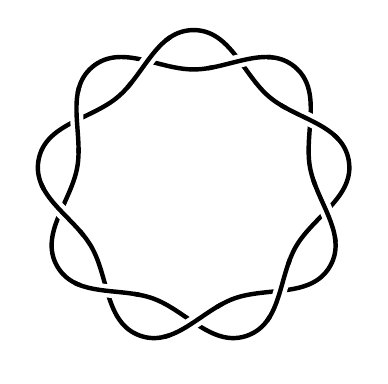
\begin{tikzpicture}[use Hobby shortcut]
                \begin{knot}[
                  consider self intersections=true,
                  flip crossing/.list={2,4,6,8,10}
                ]
                    \strand ([closed]90:2) foreach \k in {1,...,9} { .. (90-360/9+\k*720/9:1.5) .. (90+\k*720/9:2) } (90:2);
                \end{knot}
            \end{tikzpicture}
            &
            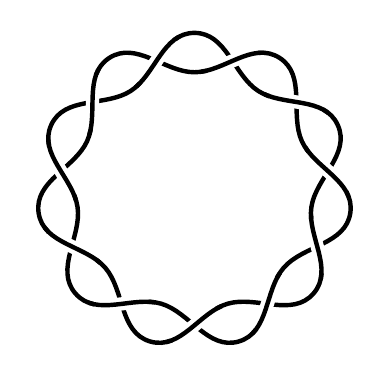
\begin{tikzpicture}[use Hobby shortcut]
                \begin{knot}[
                    consider self intersections=true,
                    flip crossing/.list={2,4,6,8,10,12}
                ]
                    \strand ([closed]90:2) foreach \k in {1,...,11} { .. (90-360/11+\k*720/11:1.5) .. (90+\k*720/11:2) } (90:2);
                \end{knot}
            \end{tikzpicture}
      \end{tabular}
    \end{table}

    \subsection{Twist Knot Ladder}
    \begin{table}[h!]
        \centering
        \caption{The $3_1$ Trefoil is the only knot that is a Torus and Twist knot}
        \label{tab:twist-torus-3-4-5}
        \begin{tabular}{c c c}
            \textbf{$\frac{1}{2}$Twist $_{(trefoil)}$} & \textbf{$\frac{2}{2}$Twist $_{(figure 8)}$} & \textbf{$\frac{3}{2}$Twists} \\
            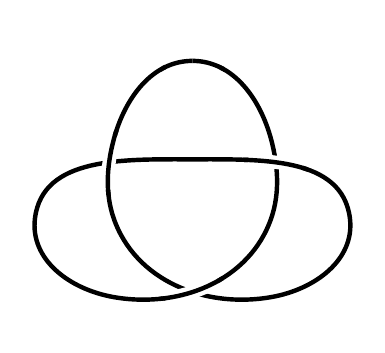
\begin{tikzpicture}[use Hobby shortcut]
                \coordinate (P1) at (0.0, 2.0);
                \coordinate (P2) at (-1.0, 1.0);
                \coordinate (P3) at (-1.0, 0.0);
                \coordinate (P4) at (1.0, -1.0);
                \coordinate (P5) at (2.0, 0.0);
                \coordinate (P6) at (0.0, 0.75);
                \coordinate (P7) at (-2.0, 0.0);
                \coordinate (P8) at (-1.0, -1.0);
                \coordinate (P9) at (1.0, 0.0);
                \coordinate (P10) at (1.0, 1.0);
                \begin{knot}[
                    consider self intersections,
                    ignore endpoint intersections=false,
                    flip crossing/.list={2,4,6,8,10,12,14},
                ]
                    \strand ([closed] P1)..(P2)..(P3)..(P4)..(P5)..(P6)..(P7)..(P8)..(P9)..(P10);
                \end{knot}
            \end{tikzpicture}
            &
            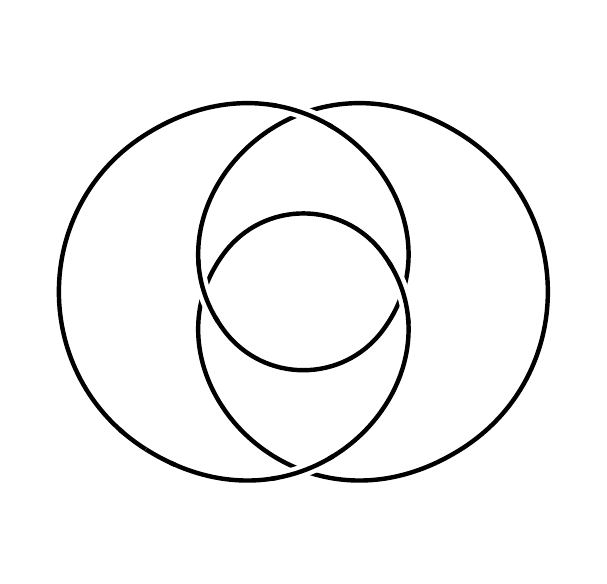
\begin{tikzpicture}[use Hobby shortcut]
                \coordinate (P1) at (-2.0, -2.0);
                \coordinate (P2) at (-2.0, 2.0);
                \coordinate (P3) at (1.0, -0.5);
                \coordinate (P4) at (-1.0, -0.5);
                \coordinate (P5) at (2.0, 2.0);
                \coordinate (P6) at (2.0, -2.0);
                \coordinate (P7) at (-1.0, 0.5);
                \coordinate (P8) at (1.0, 0.5);
                \coordinate (P9) at (-2.0, -2.0);
                \begin{knot}[
                    consider self intersections,
                    ignore endpoint intersections=false,
                    flip crossing/.list={2,4,6,8,10,12,14},
                ]
                    \strand ([closed] P1)..(P2)..(P3)..(P4)..(P5)..(P6)..(P7)..(P8)..(P9);
                \end{knot}
            \end{tikzpicture}


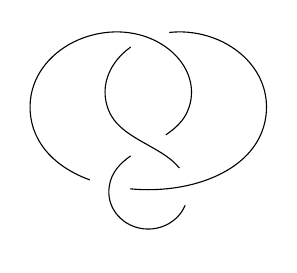
\begin{tikzpicture}[use Hobby shortcut]
\path[spath/save=figure8]
([closed]0,0) .. (1.5,1) .. (.5,2) ..
(-.5,1) .. (.5,0) .. (0,-.5) .. (-.5,0) ..
(.5,1) .. (-.5,2) .. (-1.5,1) .. (0,0);
\tikzset{
  every spath component/.style={draw},
  spath/knot={figure8}{15pt}{1,3,...,7}
}
\path (0,-.7);
\end{tikzpicture}

            &
            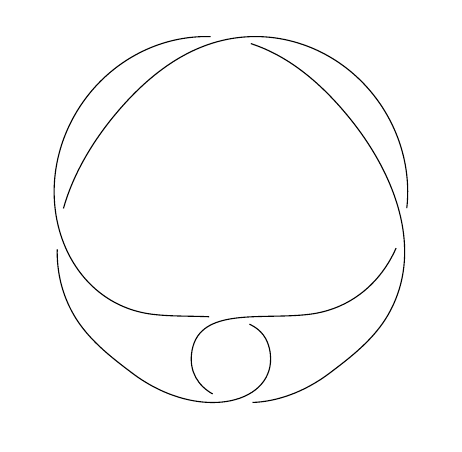
\begin{tikzpicture}[use Hobby shortcut]
                \coordinate (P1) at (2.0, -1.5);
                \coordinate (P2) at (1.5, 1.0);
                \coordinate (P3) at (0.0, 2.0);
                \coordinate (P4) at (-2.0, 1.0);
                \coordinate (P5) at (-1.0, -1.5);
                \coordinate (P6) at (0.5, -2.0);
                \coordinate (P7) at (-1.25, -2.25);
                \coordinate (P8) at (-2.0, -1.5);
                \coordinate (P9) at (-1.5, 1.0);
                \coordinate (P10) at (0.0, 2.0);
                \coordinate (P11) at (2.0, 1.0);
                \coordinate (P12) at (1.0, -1.5);
                \coordinate (P13) at (-0.5, -2.0);
                \coordinate (P14) at (1.25, -2.25);
                \coordinate (P15) at (2.0, -1.5);
                \path[spath/save=5-2]
                     ([closed] P1)..(P2)..(P3)..(P4)..(P5)..(P6)..(P7)..(P8)..(P9)..(P10)..(P11)..(P12)..(P13)..(P14)..(P15);
                \tikzset{
                    every spath component/.style={draw},
                    spath/knot={5-2}{15pt}{1,3,...,9}
                }
            \end{tikzpicture}

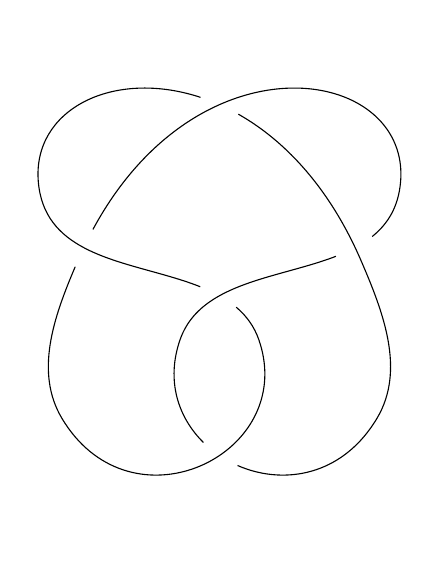
\begin{tikzpicture}[use Hobby shortcut]
\path[spath/save=5-2]
([closed]2,-2)..(1.8,0)..(-2.3,1)..(.5,-1)..(-2,-2)..(-1.8,0)..(2.3,1)..(-.5,-1)..(2,-2);
\tikzset{
  every spath component/.style={draw},
  spath/knot={5-2}{15pt}{1,3,...,9}
}
\end{tikzpicture}

        \end{tabular}
    \end{table}

    \begin{table}[h!]
        \centering
        \caption{Twist / half-twist torus knots (II)}
        \label{tab:twist-torus-6-7-8}
        \begin{tabular}{c c c}
            \textbf{$6_1$ four half-twists} & \textbf{$7_2$ twist} & \textbf{$8_1$ twist octafoil} \\
            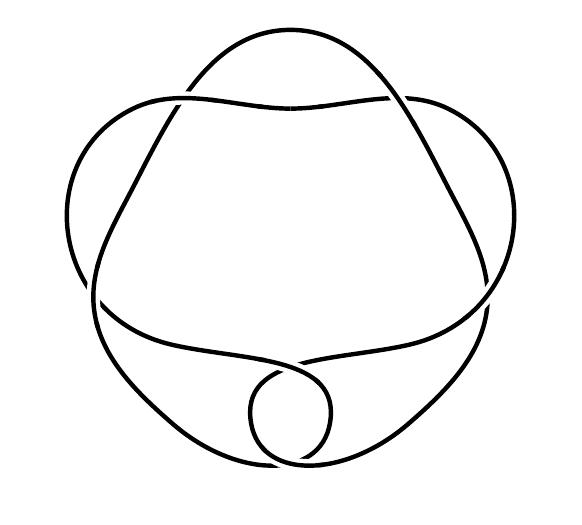
\begin{tikzpicture}[use Hobby shortcut]
                \coordinate (P1) at (0.0, 2.0);
                \coordinate (P2) at (-2.0, 2.0);
                \coordinate (P3) at (-1.5, -1.0);
                \coordinate (P4) at (0.5, -2.0);
                \coordinate (P5) at (-1.5, -2.0);
                \coordinate (P6) at (-2.5, -0.5);
                \coordinate (P7) at (-2.0, 1.0);
                \coordinate (P8) at (0.0, 3.0);
                \coordinate (P9) at (2.0, 1.0);
                \coordinate (P10) at (2.5, -0.5);
                \coordinate (P11) at (1.5, -2.0);
                \coordinate (P12) at (-0.5, -2.0);
                \coordinate (P13) at (1.5, -1.0);
                \coordinate (P14) at (2.0, 2.0);
                \coordinate (P15) at (0.0, 2.0);
                \begin{knot}[
                    consider self intersections,
                    ignore endpoint intersections=false,
                    flip crossing/.list={2,4,6,8,10,12,14,16,18},
                ]
                    \strand ([closed] P1)..(P2)..(P3)..(P4)..(P5)..(P6)..(P7)..(P8)..(P9)..(P10)..(P11)..(P12)..(P13)..(P14)..(P15);
                \end{knot}
            \end{tikzpicture}
            &
            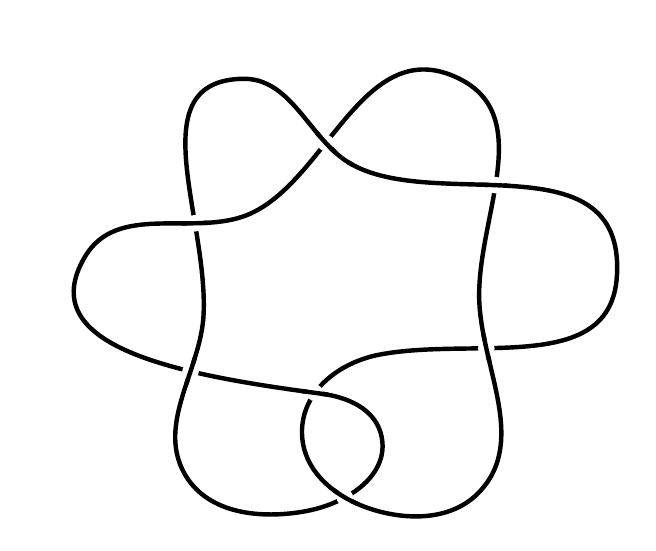
\begin{tikzpicture}[use Hobby shortcut]
                \coordinate (P1) at (0, 2);
                \coordinate (P2) at (-1.25, 3);
                \coordinate (P3) at (-1.75, 0);
                \coordinate (P4) at (-2, -2);
                \coordinate (P5) at (-0.50, -2.50);
                \coordinate (P6) at (0.50, -1.50);
                \coordinate (P7) at (-0.25, -1);
                \coordinate (P8) at (-3.25, 0.75);
                \coordinate (P9) at (-1.25, 1.25);
                \coordinate (P10) at (1.50, 3);
                \coordinate (P11) at (1.75, 0.25);
                \coordinate (P12) at (1.75, -2.25);
                \coordinate (P13) at (0.50, -2.50);
                \coordinate (P14) at (-0.50, -1.50);
                \coordinate (P15) at (0.50, -0.50);
                \coordinate (P16) at (3.50, 0.50);

                \begin{knot}[
                    consider self intersections,
                    clip width=5pt, clip radius=3pt,
                    ignore endpoint intersections=false,
                    flip crossing/.list={2,4,6,8,10,12,14,16,18,20},
                    % ----draft mode=crossings % uncomment to see numbers
                ]
                \strand
                ([closed] P1)..(P2)..(P3)..(P4)..(P5)..(P6)..(P7)..(P8)..(P9)..(P10)..(P11)..(P12)..(P13)..(P14)..(P15)..(P16);
                \end{knot}
            \end{tikzpicture}
            &
            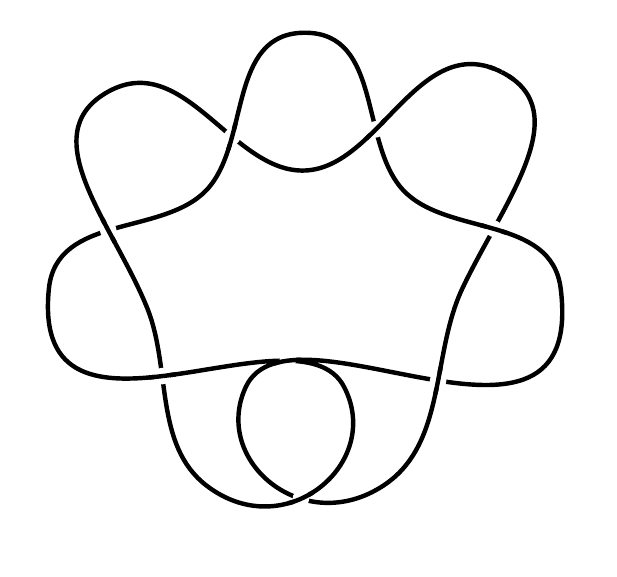
\begin{tikzpicture}[use Hobby shortcut]
                \coordinate (P1) at (2.50, 2.75);
                \coordinate (P2) at (0, 1.50);
                \coordinate (P3) at (-2.50, 2.50);
                \coordinate (P4) at (-2, -0.25);
                \coordinate (P5) at (-1.25, -2.50);
                \coordinate (P6) at (0.50, -1.25);
                \coordinate (P7) at (-3.25, 0);
                \coordinate (P8) at (-1.25, 1.25);
                \coordinate (P9) at (0, 3.25);
                \coordinate (P10) at (1.25, 1.25);
                \coordinate (P11) at (3.25, 0);
                \coordinate (P12) at (-0.75, -1.25);
                \coordinate (P13) at (1, -2.50);
                \coordinate (P14) at (2, 0);

                \begin{knot}[
                    consider self intersections,
                    clip width=5pt, clip radius=3pt,
                    ignore endpoint intersections=false,
                    flip crossing/.list={2,4,6,8,10,12,14,16,18,20},
                    % ----draft mode=crossings % uncomment to see numbers
                ]
                \strand
                ([closed] P1)..(P2)..(P3)..(P4)..(P5)..(P6)..(P7)..(P8)..(P9)..(P10)..(P11)..(P12)..(P13)..(P14);
                \end{knot}
                \end{tikzpicture}
        \end{tabular}
    \end{table}

    \begin{table}[h!]
        \centering
        \caption{Twist / half-twist torus knots (III)}
        \label{tab:twist-torus-9-10}
        \begin{tabular}{c c c}
            \textbf{$9_2$ twist} & \textbf{$10_1$ twist dekafoil} & \textbf{$11_2$ twist undecafoil} \\
            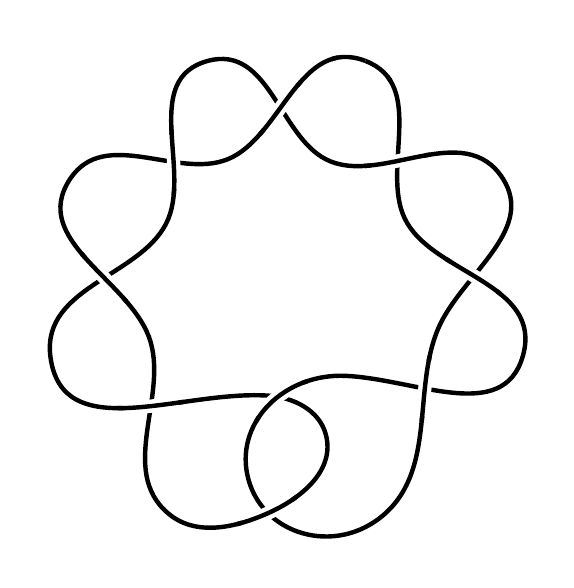
\begin{tikzpicture}[use Hobby shortcut]
                \coordinate (P1) at (0.75, 3.25);
                \coordinate (P2) at (-1.0, 2.0);
                \coordinate (P3) at (-3.0, 1.75);
                \coordinate (P4) at (-2.0, -0.25);
                \coordinate (P5) at (-1.75, -2.50);
                \coordinate (P6) at (-0.50, -2.50);
                \coordinate (P7) at (0.25, -1.50);
                \coordinate (P8) at (-0.50, -1.0);
                \coordinate (P9) at (-3.25, -0.50);
                \coordinate (P10) at (-1.75, 1.25);
                \coordinate (P11) at (-1.25, 3.25);
                \coordinate (P12) at (0.25, 2.0);
                \coordinate (P13) at (2.50, 1.75);
                \coordinate (P14) at (1.75, 0.0);
                \coordinate (P15) at (1.0, -2.50);
                \coordinate (P16) at (-0.75, -2.0);
                \coordinate (P17) at (0.50, -0.75);
                \coordinate (P18) at (2.75, -0.50);
                \coordinate (P19) at (1.25, 1.25);
                \coordinate (P20) at (0.75, 3.25);
                \begin{knot}[
                    consider self intersections,
                    ignore endpoint intersections=false,
                    flip crossing/.list={2,4,6,8,10,12,14,16,18,20},
                ]
                    \strand ([closed] P1)..(P2)..(P3)..(P4)..(P5)..(P6)..(P7)..(P8)..(P9)..(P10)..(P11)..(P12)..(P13)..(P14)..(P15)..(P16)..(P17)..(P18)..(P19)..(P20);
                \end{knot}
            \end{tikzpicture}
            &
            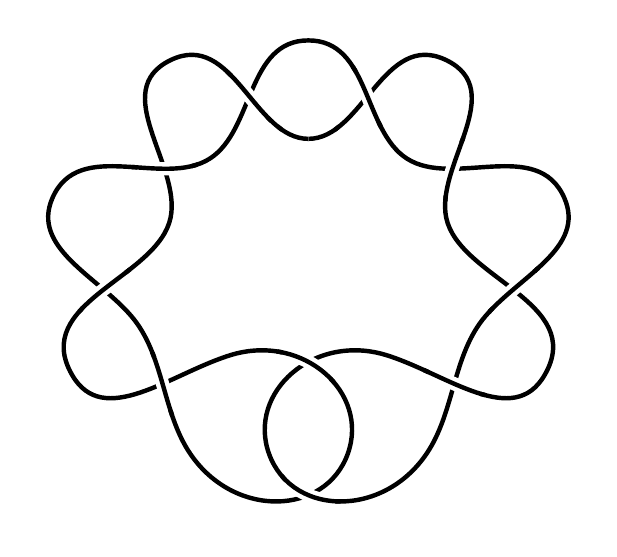
\begin{tikzpicture}[use Hobby shortcut]
                \coordinate (P1) at (0.0, 2.0);
                \coordinate (P2) at (-1.75, 3.0);
                \coordinate (P3) at (-1.75, 1.0);
                \coordinate (P4) at (-3.0, -1.0);
                \coordinate (P5) at (-1.0, -0.75);
                \coordinate (P6) at (0.50, -2.0);
                \coordinate (P7) at (-1.50, -2.0);
                \coordinate (P8) at (-2.25, -0.25);
                \coordinate (P9) at (-3.25, 1.25);
                \coordinate (P10) at (-1.25, 1.75);
                \coordinate (P11) at (0.0, 3.25);
                \coordinate (P12) at (1.25, 1.75);
                \coordinate (P13) at (3.25, 1.25);
                \coordinate (P14) at (2.25, -0.25);
                \coordinate (P15) at (1.50, -2.0);
                \coordinate (P16) at (-0.50, -2.0);
                \coordinate (P17) at (1.0, -0.75);
                \coordinate (P18) at (3.0, -1.0);
                \coordinate (P19) at (1.75, 1.0);
                \coordinate (P20) at (1.75, 3.0);
                \coordinate (P21) at (0.0, 2.0);
                \begin{knot}[
                    consider self intersections,
                    ignore endpoint intersections=false,
                    flip crossing/.list={2,4,6,8,10,12,14,16,18,20},
                ]
                    \strand ([closed] P1)..(P2)..(P3)..(P4)..(P5)..(P6)..(P7)..(P8)..(P9)..(P10)..(P11)..(P12)..(P13)..(P14)..(P15)..(P16)..(P17)..(P18)..(P19)..(P20)..(P21);
                \end{knot}
            \end{tikzpicture}
            &
                        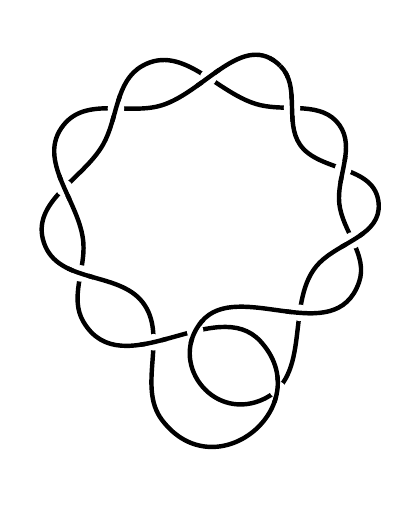
\begin{tikzpicture}[use Hobby shortcut]
    \coordinate (P1) at (0.50, 2.50);
    \coordinate (P2) at (-1, 2);
    \coordinate (P3) at (-2.25, 1.75);
    \coordinate (P4) at (-2, 0.25);
    \coordinate (P5) at (-2, -0.75);
    \coordinate (P6) at (0.25, -1);
    \coordinate (P7) at (-1, -2);
    \coordinate (P8) at (-1.25, -0.50);
    \coordinate (P9) at (-2.50, 0.25);
    \coordinate (P10) at (-1.75, 1.50);
    \coordinate (P11) at (-1.25, 2.50);
    \coordinate (P12) at (0.25, 2);
    \coordinate (P13) at (1.25, 1.75);
    \coordinate (P14) at (1.25, 0.75);
    \coordinate (P15) at (1.50, -0.25);
    \coordinate (P16) at (-0.50, -0.75);
    \coordinate (P17) at (0.25, -1.75);
    \coordinate (P18) at (1, 0);
    \coordinate (P19) at (1.75, 0.75);
    \coordinate (P20) at (0.75, 1.50);

    \begin{knot}[
        consider self intersections,
        clip width=5pt, clip radius=3pt,
        ignore endpoint intersections=false,
        flip crossing/.list={2,4,6,8,10,12,14,16,18,20,22},
        % ----draft mode=crossings % uncomment to see numbers
    ]
    \strand
    ([closed] P1)..(P2)..(P3)..(P4)..(P5)..(P6)..(P7)..(P8)..(P9)..(P10)..(P11)..(P12)..(P13)..(P14)..(P15)..(P16)..(P17)..(P18)..(P19)..(P20);
    \end{knot}
    \end{tikzpicture}
        \end{tabular}
    \end{table}



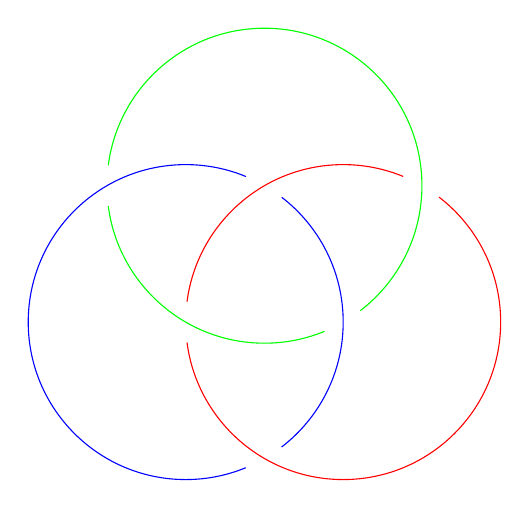
\begin{tikzpicture}
\path[spath/save=right] (1,0) circle[radius=2cm];
\path[spath/save=left] (-1,0) circle[radius=2cm];
\path[spath/save=upper] (0,{sqrt(3)}) circle[radius=2cm];
\tikzset{
  spath/remove empty components/.list={right,left,upper},
  spath/split at intersections={left}{right},
  spath/split at intersections={right}{upper},
  spath/split at intersections={upper}{left},
  spath/insert gaps after components={left}{15pt}{2,4},
  spath/insert gaps after components={right}{15pt}{1,3},
  spath/insert gaps after components={upper}{15pt}{1,3},
  spath/spot weld/.list={right,left,upper},
}
\draw[blue, spath/use={left}];
\draw[red, spath/use={right}];
\draw[green, spath/use={upper}];
\end{tikzpicture}






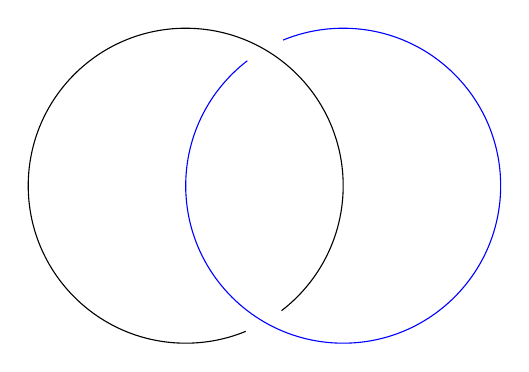
\begin{tikzpicture}
\path[spath/save=right] (1,0) circle[radius=2cm];
\path[spath/save=left] (-1,0) circle[radius=2cm];
\tikzset{
  spath/remove empty components/.list={left,right},
  spath/split at intersections={left}{right},
  spath/insert gaps after components={left}{15pt}{1},
  spath/insert gaps after components={right}{15pt}{2},
  spath/spot weld/.list={left,right},
}
\draw[spath/use={left}];
\draw[blue,spath/use={right}];
\end{tikzpicture}



\end{document}